%Autor: aplatanad & AgarFu
%aplatanad: 2
%AgarFu: 6

\chapter{Depuradores}
\label{depuradores.tex}
\index{Depuradores}
\section{Depurando la aplicación}

Se suele decir que el 10\% del  tiempo de desarrollo de un programa se
dedica a la codificación y el 90\% restante a la depuración. Al margen
de  que sea  cierto o  no la  verdad es  que es  de vital  importancia
disponer de las  herramientas adecuadas para corregir  los errores del
software en un tiempo razonable.

La primera  recomendación es  dejar que  {\tt lclint}  analice nuestro
código  para  que  busque  y notifique  cualquier  inconsistencia.  Es
importante destacar que dicho programa es mucho más potente detectando
posibles errores que  el analizador sintáctico del {\tt  gcc} debido a
que  el  compilador asume  que  ya  hemos  pasado nuestro  código  por
un  programa  como  {\tt  lclint}.  Esa  suposición  permite  al  {\tt
gcc}  realizar  ciertas optimizaciones  que  mejoran  su velocidad  de
compilación.

\begin{verbatim}
$ lclint main.c holafunc.c
\end{verbatim}

Si disponemos de nuestro programa perfectamente compilado y observamos
que  presenta algún  error del  que no  sabemos determinar  su origen,
significa  que ha  llegado la  hora utilizar  el depurador.  GNU/Linux
dispone del {\sf  GNU Debugger} bajo el  comando {\tt gdb}\label{gdb}.
Para  \index{Depuradores!GNU  Debugger   (GDB)}  usarlo  sólo  debemos
ejecutarlo  especificando  el  nombre  del programa  en  la  línea  de
comandos; y haber compilado nuestro programa con la opción {\tt -g}.

\begin{verbatim}
$ gdb holamundo
GNU gdb 2002-04-01-cvs
Copyright 2002 Free Software Foundation, Inc.
GDB is free software, covered by the GNU General Public License, and you are
welcome to change it and/or distribute copies of it under certain conditions.
Type "show copying" to see the conditions.
There is absolutely no warranty for GDB.  Type "show warranty" for details.
This GDB was configured as "i386-linux"...
(gdb) 
\end{verbatim}

En ese momento tendremos al {\tt gdb} esperando alguno de los comandos
de depuración.  A con\-ti\-nua\-ción  disponemos de  una lista  de los
comandos más básicos.

\begin{description}

\item[{\tt break}]  Sitúa un punto  de ruptura  en la línea  o función
indicada como argumento.

\item[{\tt continue}]  Continúa la ejecución  de un programa  que está
siendo depurado y se encuentra detenido en un punto de ruptura.

\item[{\tt display  exp}] Muestra el  valor de la expresión  {\tt exp}
cada vez que el programa se detiene.

\item[{\tt  help}] Lista  las clases  de comandos  disponibles. Si  el
comando va  seguido por un nombre  de clase se listan  los comandos de
dicha clase.  Si va seguido  por un nombre  de comando se  muestra una
ayuda completa del comando indicado.

\item[{\tt  list}]  Lista una  línea  o  función especificada.  Si  el
comando  va seguido  del nombre  de  una función,  el comando  muestra
dicha  función. Si  va  seguido de  un número  de  línea, muestra  esa
línea.  En  programas  de  varios  archivos  se  puede  utilizar  {\tt
nombre\_archivo:nombre\_funcion} o {\tt nombre\_archivo:numero\_línea}
para  listar  los  contenidos  de  un archivo  particular.  Si  no  se
especifican argumentos se  lista desde la última línea  mostrada; y si
se  especifican  dos números  de  línea  separados  por una  coma,  se
muestran las líneas comprendidas en el intervalo.

\item[{\tt next}] Ejecución paso a  paso pero ignorando las llamadas a
funciones.

\item[{\tt print exp}]  Muestra el valor de la expresión  {\tt exp} en
el punto actual.

\item[{\tt quit}] Salir del {\tt gdb}.

\item[{\tt run}] Inicia la ejecución  del programa. Los argumentos del
comando son los argumentos que se le pasan al programa.

\item[{\tt  step}] Ejecución  paso  a paso  incluso  de las  funciones
llamadas por el programa.

\item[{\tt undisplay  exp}] Deja de  mostrar el valor de  la expresión
{\tt exp} cada vez que el programa se detiene.

\end{description}

El  número  de  comandos  es  mucho más  grande  pero  basta  con  los
anteriores para agilizar enormemente  nuestro trabajo. Una alternativa
a todo  esto es  usar el {\tt  ddd} que se  puede considerar  como una
interfaz gráfica  para el {\tt gdb}.  Funciona sobre las {\sf  X} y su
uso es semejante a de los depuradores existentes en otras plataformas.

\section{Data Display Debugger: DDD}
\index{Depuradores!Data Display Debugger}

Como ya  hemos comentado anteriormente los  programadores suelen pasar
mucho tiempo utilizando un depuraror  para buscar fallos que no son
faciles de encontrar simplemente mirando el código, esto suele ocurrir
muy  habitualmente cuando  se trabaja  con memoria  dinámica, pues  la
asignacion de  ésta no se hace  en tiempo de compilación,  sino que se
hace en  tiempo de  ejecución y  es más  complicado seguirle  la pista
cuando estamos escribiendo código, además normalmente los analizadores
sintácticos de los compiladores no  detectan muchos de los errores que
cometemos por ser ``legales'' en determinadas circunstancias.\\

Hemos presentado el {\tt  gdb} que es muy util y  potente, de hecho es
uno de los pocos depuradores  que encontramos para los sistemas linux.
El  {\tt  gdb}  es  feo,  de  eso  tampoco  hay  duda  y  no  queremos
que  las cosas  sean tan  poco  amigables. Así  aparecen muchos  otros
programas que, utilizando  ellos el {\tt gdb}  por nosotros, consiguen
presentarnos una cara más amistosa de este fantástico depurador. Ahora
verás uno de los más laureados, el {\sf Data Display Debugger}.

\begin{figure}[hbtp]
\centering
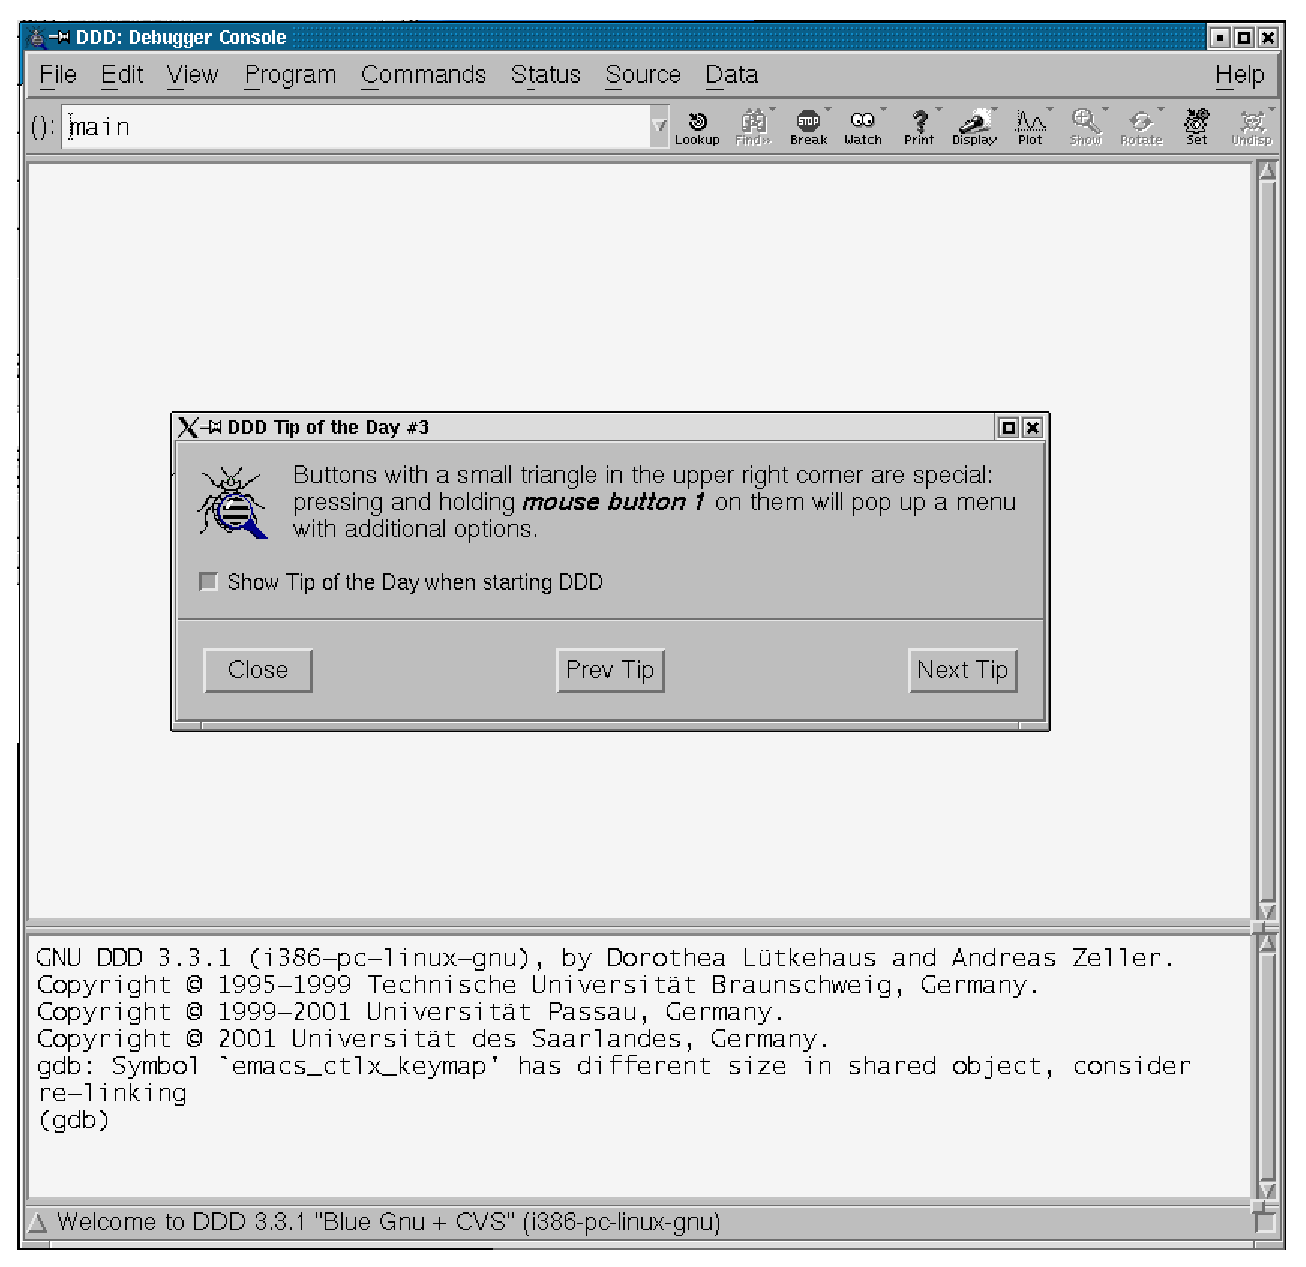
\includegraphics[width=\textwidth]{imagenes/ddd_inicio.eps}
\caption{Pantalla de inicio}
\end{figure}

Este es  el aspecto que  presenta el  {\tt ddd} cuando  lo arrancamos,
vamos a ir por pasos mostrando  lo que normalmente un programador como
nosotros vamos a necesitar de un depurador.

\subsection{Mostrar el contenido de las variables}

Para mostrar el contenido de las  variables lo que tendremos que hacer
es, como se dice coloquialmente, colocar un {\em watch} a la variable.
En {\tt ddd} esto  es muy sencillo de hacer y  hay varias maneras, una
de ellas puede ser  escribir el nombre de la variable  en el cuadro de
texto que  tenemos justo por  debajo de la barra  de menú y  pulsar el
botón de watch que está al mismo nivel un poco más a la derecha:

\begin{figure}[hbtp]
\centering
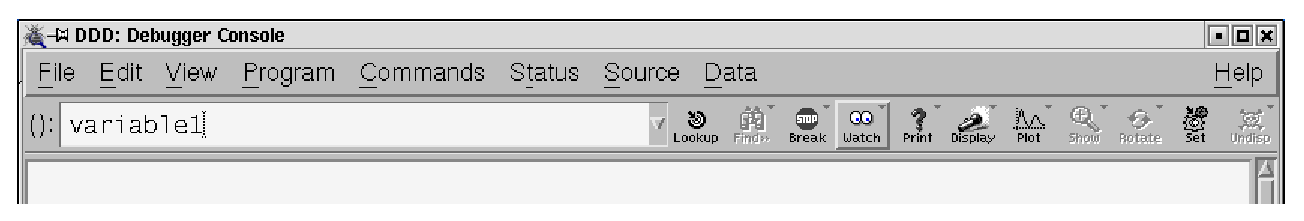
\includegraphics[width=\textwidth]{imagenes/ddd_watch.eps}
\caption{Barra de herramientas}
\end{figure}

Otra forma de hacerlo quizá más rápida poner el cursor del ratón sobre
el nombre de la variable en  el código fuente, pulsar el boton derecho
y escoger la opcion display.

\begin{figure}[hbtp]
\centering
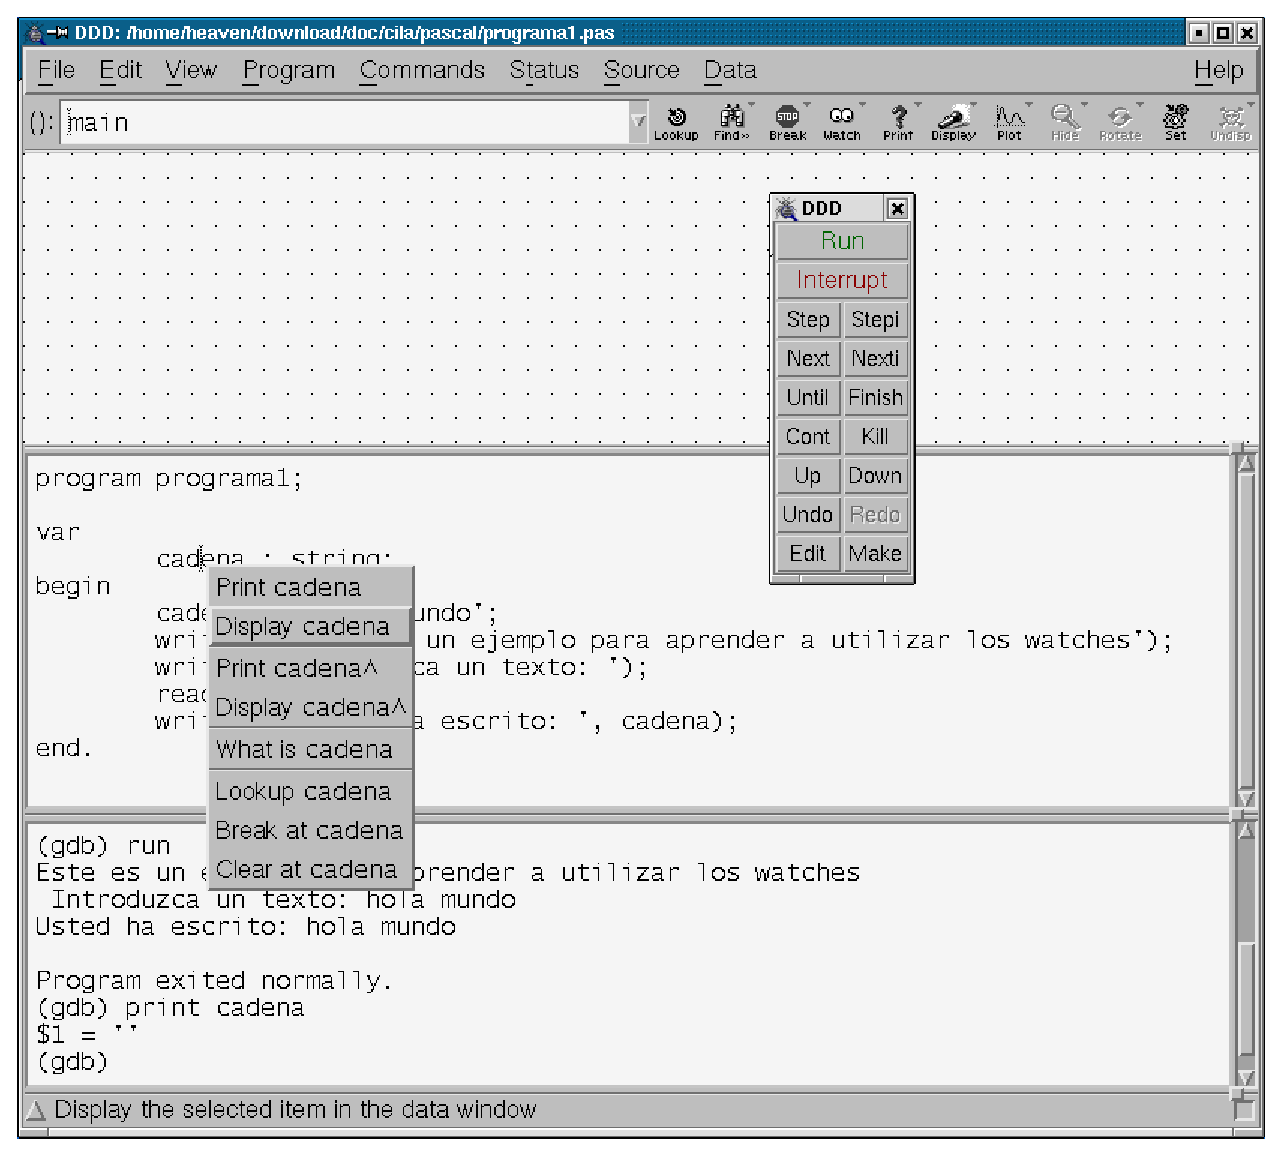
\includegraphics[width=\textwidth]{imagenes/ddd_watchII.eps}
\caption{Watches}
\end{figure}

\subsection{Colocar puntos de  ruptura (Breakpoints)}
\index{Depuradores!puntos de ruptura}

Bueno, ya tenemos un watch de la variable, pero\ldots ¿que pasa cuando
pulsamos sobre el botón de run? ¡No vemos nada! Bueno, eso es una
circunstancia pasajera, vamos a colocar un {\em punto de ruptura} o
punto de ruptura.

Los puntos de ruptura son lugares donde el depurador hará que nuestro
programa pare la ejecucuón para, de esta manera, analizar detenidamente
el estado de nuestro programa. La manera de colocar un punto de ruptura
en el {\tt ddd} es simplemente desplazarse hasta la línea donde deseamos
colocar el punto de ruptura y hacer un doble click con el boton
izquierdo del ratón.

Vemos que se nos coloca un símbolo de stop donde hemos hecho el doble
click, lo que indica que hay un punto de ruptura. Si pulsamos sobre el
punto de ruptura con el boton derecho vemos que se nos da la opcion
de desactivarlo, quitarlo y una muy extraña de propiedades. La opcion
de propiedades hace que nos aparezca un cuadro de dialogo en el cual
podemos introducir una expresión, ésta expresión se utiliza para hacer
que nuestro punto de ruptura sea inteligente y no pare la ejecución
siempre que el programa pase por allí, sino que solo se parará cuando
la expresión se cumpla, por ejemplo, si ponemos el punto de ruptura en
un bucle con 10.000 iteraciones y nosotros queremos que se pare cuando
la i (variable que cuenta las iteraciones) llegue a 5000 pues lo que
hemos de poner en propiedades del punto de ruptura es {\tt i = 5000} y
de esa manera nos saltaremos las 5000 primeras iteraciones que no nos
interesan.

\begin{figure}[hbtp]
\centering
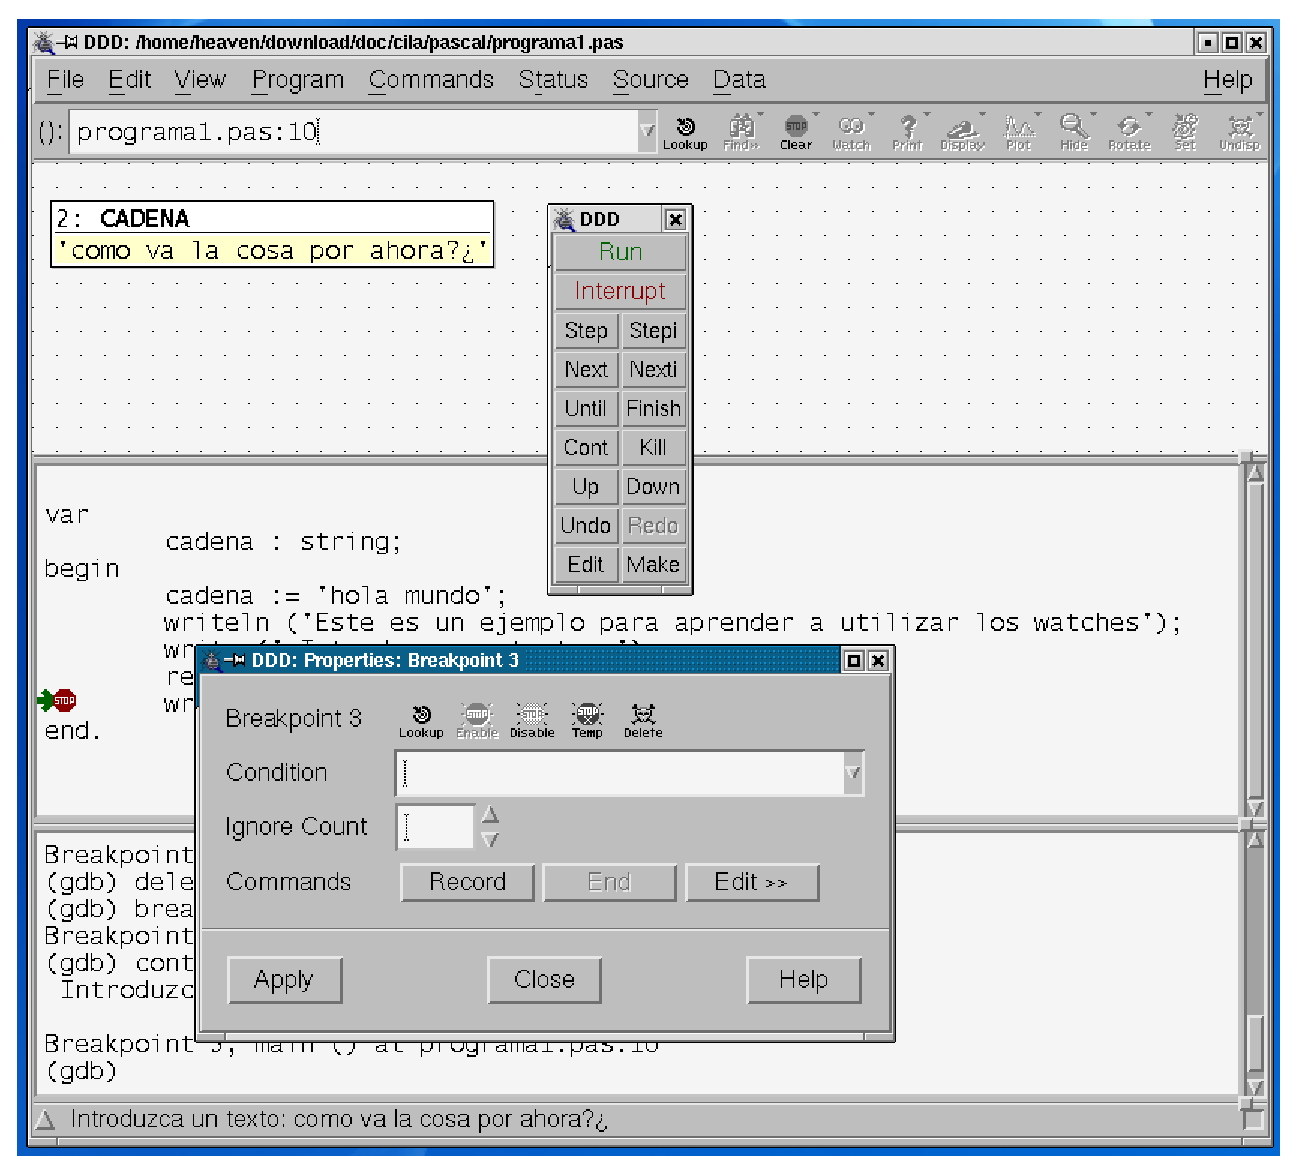
\includegraphics[width=\textwidth]{imagenes/ddd_breakpoint.eps}
\caption{Breakpoints, o puntos de ruptura}
\end{figure}

\subsection{Ejecución paso a paso}
\index{Depuradores!ejecución paso a paso}

Ahora que ya tienes un watch y un punto de ruptura, en este momento
solo podemos ir saltanto de punto de ruptura en punto de ruptura, y
esto no nos es suficiente así que vamos a intentar controlar más el
flujo de ejecución de nuestros programas. Para esta tarea tenemos varias
herramientas comunes en la mayoría de depuradores, en el caso del dd las
encontramos en una ventana que tenemos flotando sobre el depurador, con
lo cual no es complicado utilizarlas, siempre las tenemos a mano y son
las siguientes:

\begin{description}

\item[{\em Step}:]{(paso) esta herramienta nos sirve, como su propio
nombre indica, para ejecutar nuestro programa paso a paso. Normalmente
lo que hacemos es colocar un punto de ruptura al inicio de la funcion o
procedimiento que queremos analizar y luego ir pulsando {\tt step} para
analizar sentencia a sentencia que es lo que hace nuesto código.}

\item[{\em Next}:]{(siguiente) muy parecida a step, solo que pulsando
{\tt next} si en el código hay una llamada a una funcion o procedimiento
no entramos en ella, sino que ejecuta ésta y nos colocamos en la
siguiente línea del programa.}

\item[{\em Until}:]{(hasta) esta herramienta nos sirve para ejecutar el
programa hasta la posición actual del cursor, es muy parecida a un punto
de ruptura temporal.}

\item[{\em Cont}:]{(continuar) saltamos hasta el siguiente punto de
ruptura o hasta el final del programa si es que no hay ningún punto de
ruptura más en el flujo de ejecución.}

\end{description}

A  parte de  estas  herramientas  tenemos algunas  más  que se  suelen
utilizar  menos, por  ejemplo  aquellas que  ejecutan exactamente  una
instrucción (de código máquina).

\subsection{Visión de punteros}
\index{Depuradores!visión de punteros}

Probablemente estabas deseando que existiera  una cosa como la que vas
a ver. No te asombres de la  potencia de este depurador, es uno de los
pocos que lo  hacen y de ahí  viene su buena fama. La  capacidad de la
que hablamos es la de {\em ver} los punteros.

Seguramente has hecho  más de un programa con memoria  dinámica que no
acababa de  funcionar bien porque se  te perdían punteros y  no sabias
muy bien  por donde andaban  o a  dónde estaban apuntando,  pues bien,
esto ya no es excusa para entregar una práctica a medio hacer, el {\tt
ddd} viene en nuestra ayuda  y tenemos la {\em herramienta definitiva}
para la depuración con punteros.\\

Cuando  haces un  watch de  una  estructura (record)  salen todos  los
campos en un  recuadro y los punteros también salen  como otro tipo de
dato  cualquiera. Cuando  tienes {\tt  \$0}  en la  información de  un
puntero quiere  decir que  el puntero  es {\tt  Nil} (nulo),  y cuando
tenemos un número  precedido del símbolo {\tt \$} quiere  decir que el
puntero está apuntando  a esa zona de memoria, por  lo tanto, podremos
mostrar el  contenido de esa  zona de memoria. Si  decidimos mostrarla
aparecerá  otro cuadro,  como  el que  inicialmente  teníamos, con  la
información de  la zona de memoria  apuntada por el puntero  que hemos
decidido expandir  y una  flecha desde el  recuadro original  hasta el
nuevo, marcada con el nombre del puntero expandido.

De  esta manera  es  muy sencillo  seguir  los punteros  y  ver a  que
posiciones están apuntando, ver si  estamos asignando cosas a punteros
que son nulos así como que pinta va teniendo la estructura que estamos
construyendo en memoria, lo cual ayuda  mucho a la hora de moverse por
las estructuras que fabricamos.

Un ejemplo  de lo  que se puede  hacer es mostrar  un árbol  para, por
ejemplo, comprobar que todos los  punteros que salen de nuestros nodos
hoja están  a {\tt  Nil} y  de esa manera  asegurarnos de  que nuestro
programa no va a fracasar.

\begin{figure}[hbtp]
\centering
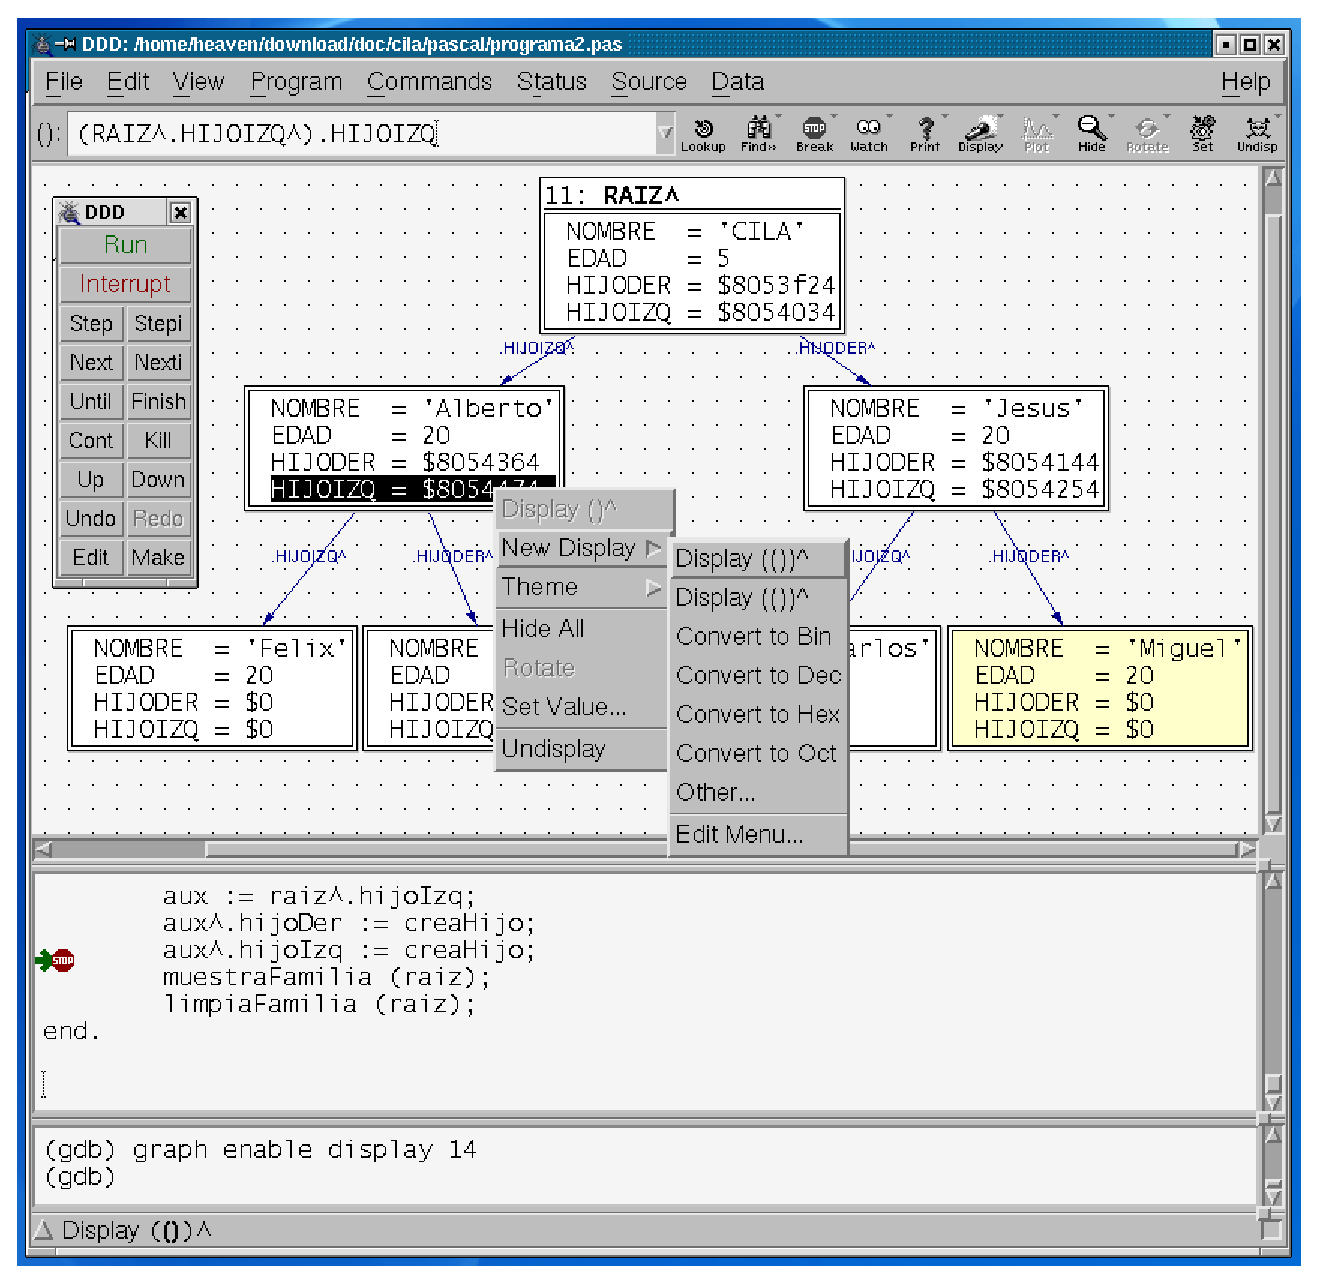
\includegraphics[width=\textwidth]{imagenes/ddd_punteros.eps}
\caption{Estructura de un árbol binario}
\end{figure}
